\documentclass{article}
\usepackage[utf8]{inputenc}
\usepackage{amsmath}
\usepackage{amsfonts}
\usepackage{graphicx}
\usepackage{multicol}
\usepackage{float}
\usepackage{cite}
\usepackage{url}
\usepackage{listings}
\usepackage{pythonhighlight}

\begin{document}
	\begin{titlepage}
		\begin{center}
			{\huge\textbf{Instituto Politécnico Nacional}}\\
			\vspace{7mm}
			{\huge\textbf{Escuela Superior de Cómputo}}\\			
			\begin{figure}[h]
				\centering
				
\includegraphics[height = 6cm]{logoEscom.png}
			\end{figure}	
			\vspace{1cm}
			{\huge\textbf{Programa 8: Gramática NO Ambigua}}
			\par\vspace{2cm}
			\large\textbf{Autor: Colín Ramiro Joel}
			\par\vspace{1cm}
			{\large\textbf{Materia: Teoría de la Computación}}
			\par\vspace{1cm}
			{\large\textbf{Grupo: 4CM2}}
			\par\vspace{1cm}
			{\large\textbf{Profesor: Juarez Martínez Genaro}}
			\par\vspace{1cm}
			{\large\textbf{Fecha de entrega: {\huge{29 de Diciembre 2021}}}}
			\par\vspace{3cm}
		\end{center}
	\end{titlepage}
	
	
	\section*{Introducción}
	La Gramática NO ambigua se refiere a aquella Gramática Libre de Contexto(GLC) para la que cada cadena válida tiene una única derivación a la izquierda, al contrario de su complemento que sería la Gramática ambigua, este tipo de gramática tiene la misma definición, unicamente que en este caso, existe una cadena que puede tener \textbf{más de una} derivación a la izquierda.
	La mayoría de los lenguajes tienen la capacidad de admitir ambos tipos de gramáticas, mientras que otros lenguajes admiten solo gramáticas ambiguas. Cualquier lenguaje no vacío admite una gramática ambigua al tomar una gramática no ambigua e introducir una regla duplicada. Por otro lado, un lenguaje que solo admite gramáticas ambiguas se conoce como un Lenguaje \textbf{Inherentemente} Ambiguo, y existen lenguajes libres del contexto inherentemente ambiguos. 
	Las gramáticas libres del contexto deterministas son no ambiguas en todo momento y son una subclase importante de Gramáticas libres de Contexto no ambiguas; existen GLCs no-deterministas y no-ambiguas simultáneamente.
	
	\section*{Instrucciones}
	Elaborar un programa para procesar la gramática no-ambigua:
	
	B $\rightarrow$(RB $\mid$ $\epsilon$
	
	R $\rightarrow$) $\mid$ (RR
		
	
	Consultar las condiciones de evaluación como están en las láminas que se vieron en la clase.
		
	Adicionalmente, el programa debe de contar con las siguientes características:
	
	\begin{enumerate}
		\item La cadena puede ser ingresada por el usuario o generada automáticamente.
		\item Mandar a un archivo y/o en pantalla la evaluación de la gramática imprimiendo el símbolo que está evaluando, indicando que producción se aplicó y la cadena generada.
		\item La longitud máxima será manejar cadenas de 1,000 caracteres.
		
	\end{enumerate}
	\section*{Desarrollo}
	Este programa se desarrolló bajo las condiciones revisadas en clase. Para esto, se implementó una función llamada \textbf{evaluacion()} a la cual se le pasa un argumento cuyo valor será la opción seleccionada por el usuario, si requiere el modo manual, introducirá el número 1 y si requiere el programa automático, introducirá el número 2. Adicionalmente, el usuario tiene la opción de salir del programa, unicamente deberá oprimir el número 3.
	
	Ahora bien, para la implementación de la función antes mencionada se requirió primero que nada un condicional if, el cual dependiendo de la opción seleccionada por el usuario, desplegará en pantalla un mensaje. En caso de que la opción selccionada sea automática, se implementó un bloque de código con la función \textbf{randint}, la cual genera una cadena de paréntesis en un rango de 1 a 1000 que es lo máximo que se requiere en el programa. 
	
	Para concluir con el desarrollo del programa, se requirió de un ciclo \textbf{for} el cual iterará desde 0 hasta la longitud de la cadena que se evalua. Posteriormente, el funcionamiento del programa es básciamente verificar si la cadena de parentésis evaluada, se encuentra en un estado balanceado o no.
	 
	\section*{Capturas del Funcionamiento}
	En esta sección se encuentran las capturas de pantalla del funcionamiento del programa, tanto de la consola, como de los archivos generados.
	Las capturas se ordenaron comforme a la opción selecionada en el programa: 
	\begin{enumerate}
		\item \textbf{Modo Manual}
		\begin{itemize}
			\item 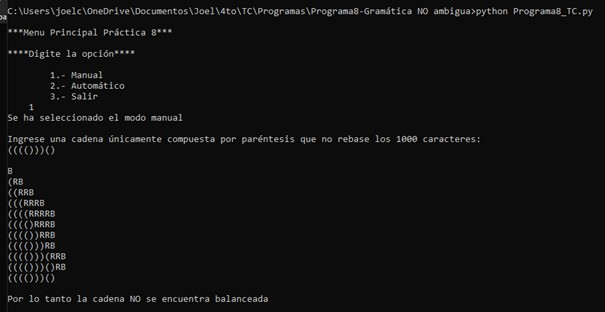
\includegraphics[height = 4cm]{MM1.jpg}
			\item 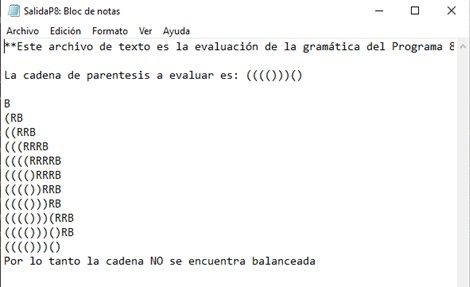
\includegraphics[height = 4cm]{MM2.jpg}			
		\end{itemize}				
		\item \textbf{Modo Automático}
		\begin{itemize}
			\item 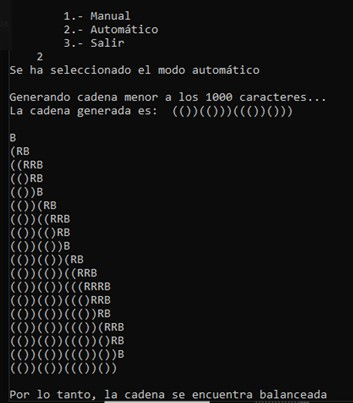
\includegraphics[height = 4cm]{MA1.jpg}
			\item 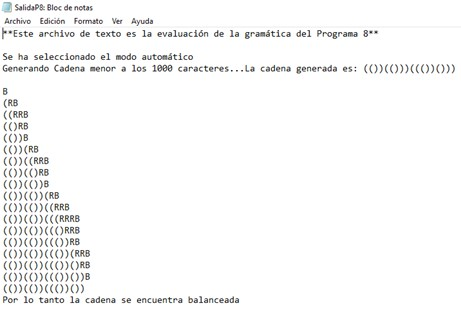
\includegraphics[height = 4cm]{MA2.jpg}			
		\end{itemize}
	\end{enumerate}
	\section*{Código}
	\begin{python}
		# Programa 8.Gramática NO Ambigua
		# Nombre: Colín Ramiro Joel
		# Profesor: Juarez Martínez Genaro
		# Grupo: 4CM2
		# Materia: Teoría Computacional
		
		from random import randint
		
		def evaluacion(opcion):
		archivo = open("SalidaP8.txt","w")
		archivo.write("**Este archivo de texto es la evaluación de la gramática del Programa 8**\n\n")
		if(opcion == 1):
		print("Se ha seleccionado el modo manual\n")
		print("Ingrese una cadena únicamente compuesta por paréntesis que no rebase los 1000 caracteres: ")
		cadenaParentesis = input()
		archivo.write("La cadena de parentesis a evaluar es: " + cadenaParentesis)
		elif(opcion == 2):
		print("Se ha seleccionado el modo automático\n")
		print("Generando cadena menor a los 1000 caracteres...")
		archivo.write("Se ha seleccionado el modo automático\n")        
		archivo.write("Generando Cadena menor a los 1000 caracteres...")  
		cadenaParentesis = " "
		longCadenaAuto = randint(1,100)
		for i in range(0, longCadenaAuto):
		aleat = randint(0,1)
		if(aleat == 0):
		cadenaParentesis = cadenaParentesis + '('
		elif(aleat == 1):                 
		cadenaParentesis = cadenaParentesis + ')'
		print("La cadena generada es: "+ cadenaParentesis)
		archivo.write("La cadena generada es:" + cadenaParentesis)   
		
		print("")
		archivo.write("\n ")
		longCadena = len(cadenaParentesis)
		finEv = "B"
		resFinal = ""
		print("B")
		archivo.write("\nB")
		for i in range(0,longCadena):        
		if(finEv[0] == "B"):
		if(cadenaParentesis[i] == "("):
		finEv = "R" + finEv
		resFinal = resFinal + "("
		print(resFinal + finEv)
		archivo.write("\n" + resFinal + finEv)
		continue                 
		if(finEv[0] == "R"):
		if(cadenaParentesis[i] == "("):
		finEv = "R" + finEv
		resFinal = resFinal + "("
		print(resFinal + finEv)
		archivo.write("\n" + resFinal + finEv)
		continue            
		if(cadenaParentesis[i] == ")"):
		finEv = finEv[1:len(finEv)]
		resFinal = resFinal + ")"
		print(resFinal + finEv)
		archivo.write("\n" + resFinal + finEv)
		continue
		if(finEv == "B"):
		print(resFinal)
		print("\nPor lo tanto, la cadena se encuentra balanceada")
		archivo.write("\n" + resFinal)
		archivo.write("\nPor lo tanto la cadena se encuentra balanceada")
		elif(finEv != "B"):
		print(resFinal)
		print("\nPor lo tanto la cadena NO se encuentra balanceada")
		archivo.write("\n" + resFinal)
		archivo.write("\nPor lo tanto la cadena NO se encuentra balanceada")
		
		opc = 0
		salir = 3
		while opc != salir:
		print("\n***Menu Principal Práctica 8***\n")
		print("****Digite la opción****")
		opc = int(input('''
		1.- Manual
		2.- Automático
		3.- Salir
		'''))  
		if(opc == 1 or opc == 2):
		evaluacion(opc)   
		elif opc == 3:
		print("Saliendo del Programa. Hasta Luego!!!!")
		else:
		print("Opcion inválida, Vuelva a intentar")
	\end{python}
	\section*{Conclusiones}
	La realización de este programa, me resultó un poco complejo, debido a que no comprendí muy bien que es lo que se debia realizar. Sin embargo, después de revisar las laminas revisadas en clase, fue más sencillo tanto de entender como el funcionamiento que debia tener el mismo.
	
	Puedo concluir que este tema de la Gramática NO ambigua es muy importante de comprender en las ciencias de la computación. Después de la realización del programa se puede observar que todos y cada uno de estos tienen mucho que ver en la construcción de un compilador, materia que se llevará más adelante en la formación como Ingeniero en Sistemas.
	
	\section*{Referencias}
	\begin{enumerate}
		\item Hopcroft, John; Motwani, Rajeev; Ullman, Jeffrey (2001). Introduction to automata theory, languages, and computation (2nd edición). Addison-Wesley. Theorem 9.20, pp. 405–406. ISBN 0-201-44124-1.
		\item Facultad de Informática . (2013). Ambigüedad. Árboles de derivación. Gramáticas ambiguas. Diciembre 21,2021, de Universidad Complutense de Madrid Sitio web: http://antares.sip.ucm.es:8180/webtalf/index.jsp?submenu=temas/submenuIncontextualescontenido=temas/ambiguedad
		\item Gonzalo Hernández Hernández. (2017). Gramáticas Ambiguas. Diciembre 21,2021, de Universidad Autónoma del Estado de Hidalgo Escuela Superior de Huejutla Sitio web: https://www.uaeh.edu.mx/docencia/P_Presentaciones/huejutla/sistemas/2017/Gramaticas_Ambiguas.pdf
		
	\end{enumerate}
	
\end{document}